\documentclass[10pt,fleqn]{article} % Default font size and left-justified equations
\usepackage[%
    pdftitle={Centrale Supelec 2018},
    pdfauthor={UPSTI}]{hyperref}

\input{style/new_style}
\input{style/macros_SII}
\usepackage{multicol}
\usepackage{siunitx}
%\usepackage{picins}
\fichetrue
%\fichefalse

\proftrue
\proffalse

%\tdtrue
\tdfalse

\courstrue
\coursfalse

% -------------------------------------
% Déclaration des titres
% -------------------------------------

\def\discipline{Sciences \\Industrielles de \\ l'Ingénieur}
\def\xxtete{Sciences Industrielles de l'Ingénieur}


\def\classe{\textsf{UPSTI}}
\def\xxnumpartie{CCS 2018}
\def\xxpartie{Modéliser le comportement statique des systèmes mécaniques}

\def\xxnumchapitre{}%Révision 1 \vspace{.2cm}}
\def\xxchapitre{Concours Centrale Supelec PSI 2018}

\def\xxposongletx{2}
\def\xxposonglettext{1.45}
\def\xxposonglety{16}%16

\def\xxonglet{\textsf{Rév -- Stat}}

\def\xxactivite{TD 01}
\def\xxauteur{\textsl{UPSTI}}


\def\xxtitreexo{Tour en fosse utilisé pour le reprofilage des roues ferroviaires}
\def\xxsourceexo{\hspace{.2cm} \footnotesize{Concours Centrale Supelec PSI 2018}}

\def\xxcompetences{%
\textsl{%
%\textbf{Savoirs et compétences :}\\
}}

\def\xxfigures{
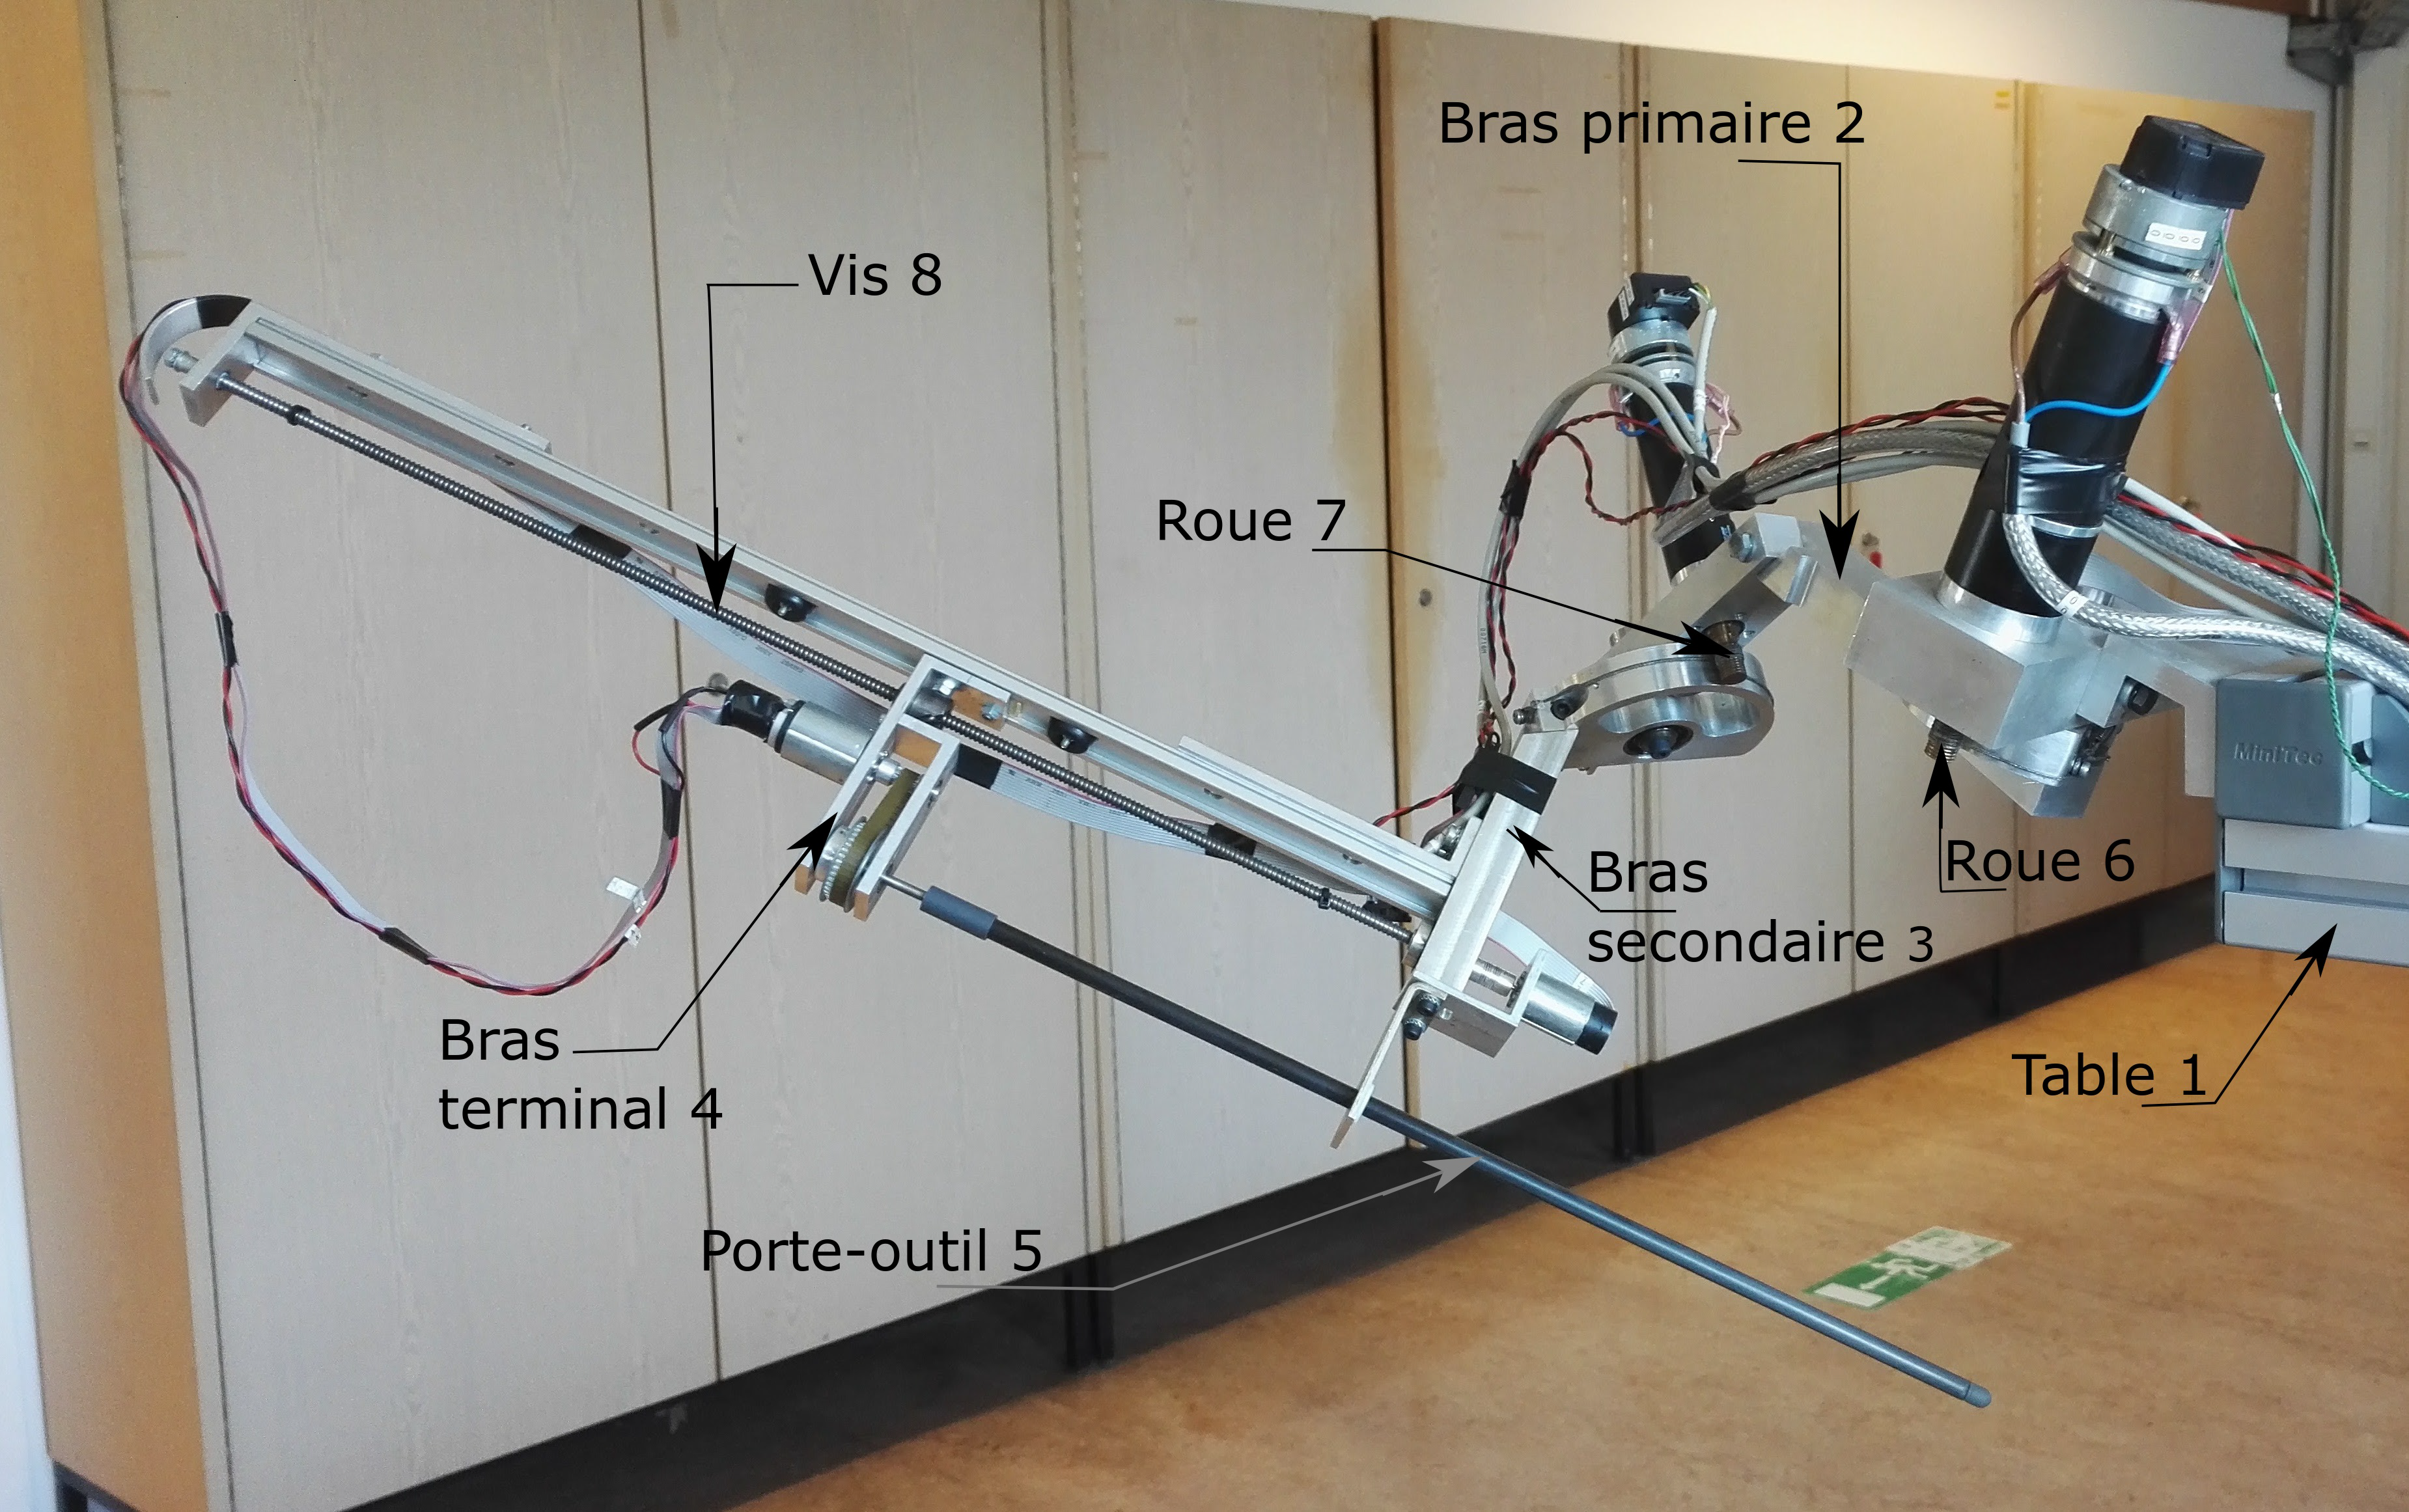
\includegraphics[width=.55\textwidth]{images/fig_00}
}%figues de la page de garde

\def\xxpied{%
Tour en fosse utilisé pour le reprofilage des roues ferroviaires\\
Concours Centrale Supelec -- PSI 2018%
}

\setcounter{secnumdepth}{5}
%---------------------------------------------------------------------------

\usepackage{bm}
\begin{document}
%\chapterimage{png/Fond_Cin}
\input{style/new_pagegarde}
\vspace{4.5cm}
\pagestyle{fancy}
\thispagestyle{plain}


\def\columnseprulecolor{\color{ocre}}
\setlength{\columnseprule}{0.4pt} 

\section{Contexte et étude préliminaire}

\begin{obj}
Valider la pertinence de l’utilisation d’une machine spéciale appelée tour en fosse pour le reprofilage
des roues ferroviaires.
\end{obj}

\subparagraph{}

\begin{itemize}
\item Pour la méthode $a$, $t_{i1} = t_3 +t_4 = \SI{14}{h}= \SI{840}{min}$.
\item Pour la méthode $b$, $t_{i2} = \left( 6\times 3 \times 2 \right)t_5 +t_6 = \SI{545}{min}$.
\end{itemize}

Le gain de temps $\Delta t_i = t_{i1}-t_{i2}=\SI{295}{min}$ soit \SI{4}{h} et \SI{55}{min}. C'est autant de temps gagner sur l'exploitation de la rame. 


.

\section{Analyse de l’entrainement en rotation d’une roue}
\subsection{Description fonctionnelle et structurelle du tour en fosse}
\subsection{Modélisation du dispositif de mise en rotation d’une roue}


\begin{obj}
Vérifier que la modélisation et les hypothèses retenues permettent de déterminer toutes les actions mécaniques nécessaires pour dimensionner les actionneurs des chaines d’énergie.
\end{obj}

\subparagraph{}

À partir des informations données, on peut réaliser le graphe de structure suivant. 

\begin{center}
\includegraphics[width=.7\linewidth]{images/fig_01}
%\textit{}
\end{center}
\begin{multicols}{2}
\textbf{Méthode cinématique}
\begin{itemize}
\item Nombre cyclomatique $\gamma = L-S+1 $ avec $L=9$ liaisons et $S=7$ solides, on a donc $\gamma = 9-7+1=3$.
\item Nombre d'inconnues cinématiques : 
\begin{itemize}
\item 2 liaisons sphériques : $3\times 2=6$ inconnues;
\item 4 liaisons pivot : $1\times 4=4$ inconnues;
\item 1 liaison pivot glissant : 2 inconnues;
\item 2 liaisons sphère-plan : $5\times 2=10$ inconnues;
\item \textbf{au total : 22 inconnues cinématiques}.
\end{itemize}
\end{itemize}
\textbf{Méthode statique}

\end{multicols}

\end{document}

\subparagraph{}\textit{}


\begin{center}
\includegraphics[width=\linewidth]{images/img_04}
%\textit{}
\end{center}

